\chapter{背景知识与相关工作}

\section{背景知识}

\subsection{线条的概念与分类}
\label{sec:diff_geo}

在一些传统的艺术效果中,例如笔墨风格和技术说明书风格,线条的绘制是很重要的一部分。为了实现这类艺术效果,计算机图形学的研究者们提出了多种不同的算法来实现基于三维模型的线绘制。根据视点相关性,可以将线绘制所讨论的线条类型分为\vdl{}(view-dependent lines)和\vidl{}(view-independent lines)两种。

本文主要讨论的\con{}和\scon{}都属于\vdl{}。在\vdl{}中,\con{}和\scon{}是最为常用的线条类型。简单来说,\con{}表示的就是几何物体的外形的凸出部分所形成的线条。在计算机图形学领域中,常用的三维模型由三角形网格构成。具体地,\con{}就是由三维模型上视线方向和表面法线的点积为零的点所组成的线。\scon{}也是一种\vdl{},它是对\con{}的补充和视觉上的延伸。

\vidl{}也是表现几何体表面的重要特征,与\vdl{}不同的是,\vidl{}只与三维模型本身的几何性质有关。计算机图形学的研究者们已经提出了各种各样的\vdl{},例如Ohtake等人提出的\cite{ohtake2004ridge}岭线(ridge)和谷线(valley)和Yoshizawa等人提出的峰线(crest)\cite{yoshizawa2005fast}。三维模型表面的折痕和模型与模型之间相交形成的交线也属于\vidl{}。由于\vidl{}和视点无关,所以它们自然是\stc{},因此本文不会对它们进行进一步的讨论。

\subsection{轮廓线的数学定义}

为了对三维模型表面的线条作出严格的、公式化的定义,计算机图形学的研究者们使用了微分几何领域的数学语言来对线条的定义进行表述。顾名思义,这个领域涉及到对曲线和表面的“微分”。对于一般的图形学研究者而言,表面法线(normal)这个概念并不陌生,它用于表示垂直于某平面的方向,广泛地用于各种绘制模型的公式之中。从微分几何的角度来看,法线其实就是表面的一阶微分。正如上一小节所述,\con{}的出现决定于法线和视线的点积是否为零。假设$N$表示表面法线,$V$表示视线方向,\con{}的决定条件即为$N\cdot{V} = 0$。类似地,其他各式各样的线条,例如\scon{},也有着和表面微分相关的数学定义,不过与之相关的是更加高阶的表面微分。

\begin{figure}[tbh]
    \centering
    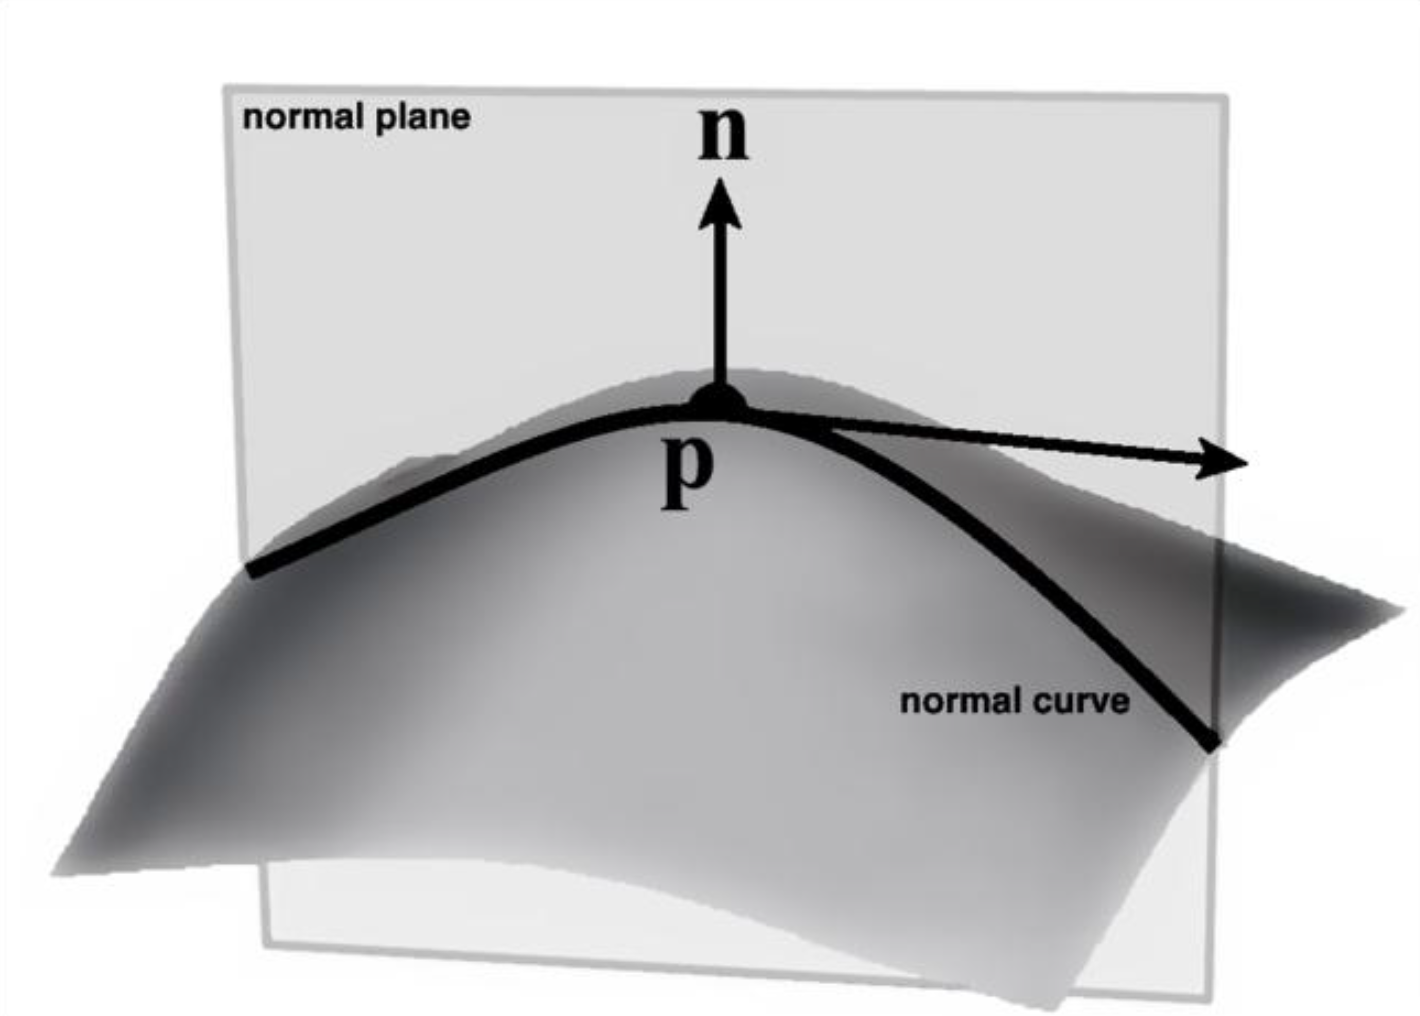
\includegraphics[width=0.6\linewidth]{normal_curvature}
    \caption[法向曲线与法向曲率]{\label{fig:normal_curvature}
    法向曲线与法向曲率\cite{rusinkiewicz2008line}}
\end{figure}

简单来说,三维模型表面的二阶微分其实就是表面对应的曲率。一般常见的曲率定义与曲线相关,它表示曲线上某一点处最逼近曲线变化的圆的半径的倒数。曲线越是弯曲,曲率的值越高。对于表面而言,可以通过用包含法线的任意平面与之相交得到一条曲线,称为法向曲线(normal curve),而对应于法向曲线的曲率便是法向曲率(normal curvature)。\autoref{fig:normal_curvature}展示了法向曲率的一个例子。对于表面上的每个点,都存在多个不同的曲率,每个曲率对应于形成法向曲线所用的不同的包含该法线的平面。

\begin{figure}[tbh]
    \centering
    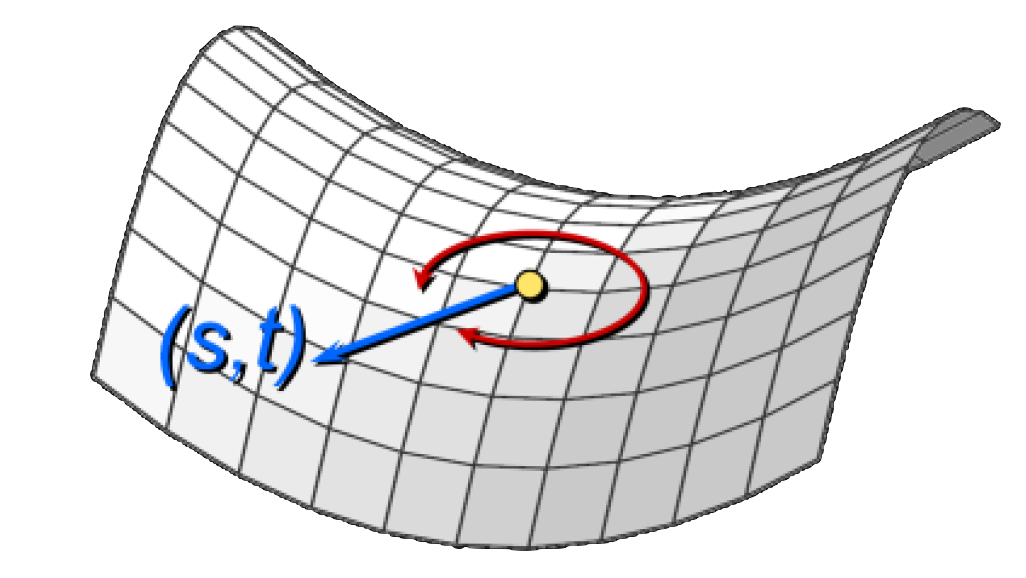
\includegraphics[width=0.6\linewidth]{sym_mat}
    \caption[某个方向上的法向曲率]{\label{fig:sym_mat}
    某个方向上的法向曲率\cite{rusinkiewicz2008line}}
\end{figure}

对于一个平滑的表面,法向曲率及其对应方向的变化不是随机的,可以用一个特定的公式表示。如\autoref{fig:sym_mat}所示,假设以表面上某点的切平面建立局部的正交坐标系,对于平面上的每个方向$(s,t)$,可以找到该方向上对应的法线曲率,其表达形式与一个对称矩阵$\rm II$有关:

\begin{equation}
    \begin{split}
        \kappa_r &= 
        \begin{pmatrix}
            s & t
        \end{pmatrix}
        \begin{pmatrix}
            e & f \\
            f & g
        \end{pmatrix}
        \begin{pmatrix}
            s \\
            t
        \end{pmatrix} \\
        &= 
        \begin{pmatrix}
            s & t
        \end{pmatrix}
        \rm II
        \begin{pmatrix}
            s \\
            t
        \end{pmatrix} \\
        &= 
        \rm II((s, t), (s, t))
    \end{split}
\end{equation}

矩阵$\rm II$表达了表面的弯曲程度。在大多数的讨论中,为了简单起见,会将局部坐标系旋转使得$\rm II$是一个对角矩阵,而新的坐标轴则是$\rm II$的特征向量。

\begin{equation}
    \rm II = R^T
    \begin{pmatrix}
        \kappa_1 & 0 \\
        0 & \kappa_2
    \end{pmatrix}
    R
\end{equation}

\begin{figure}[tbh]
    \centering
    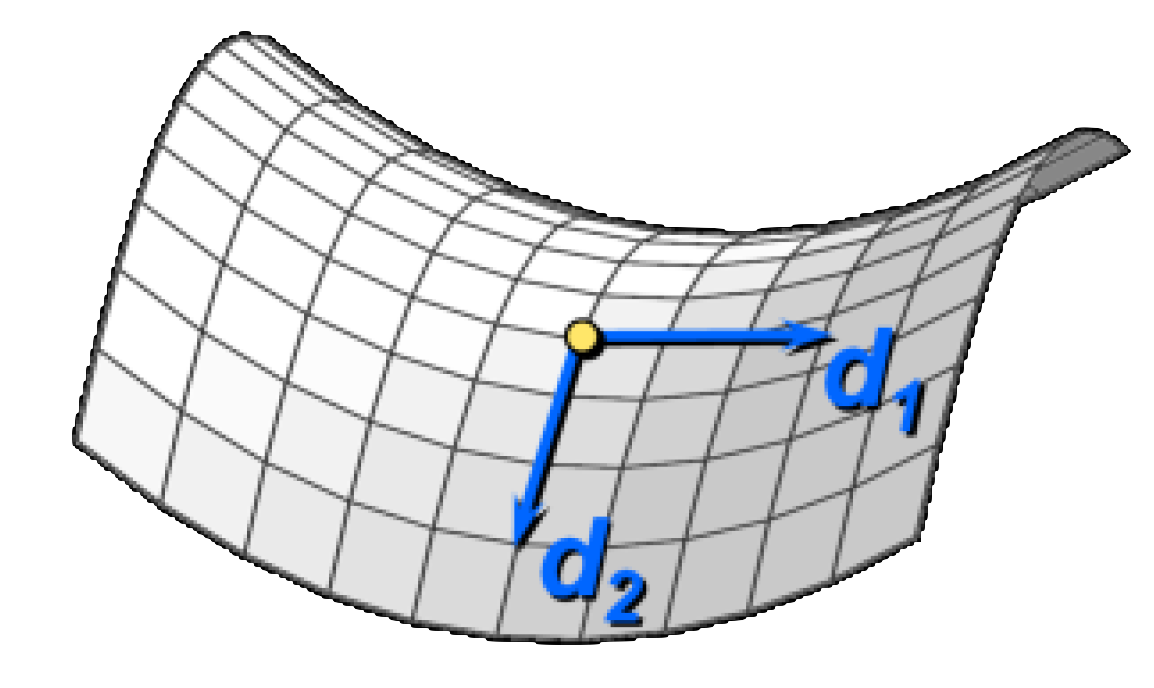
\includegraphics[width=0.6\linewidth]{sym_mat2}
    \caption[主方向与主曲率]{\label{fig:sym_mat2}
    主方向与主曲率\cite{rusinkiewicz2008line}}
\end{figure}

如\autoref{fig:sym_mat2}所示,在完成坐标系的转换后,新的坐标轴被称为主方向(principal direction),对应方向上的曲率被称为主曲率(principal curvature)。按照对应曲率的大小,两个主曲率又可以分别称为最小曲率和最大曲率,因为经过该点的所有曲率的值的大小都会在两个主曲率的值之间。具体而言,该点上沿着表面某个切线方向的法向曲率可以表示为:

\begin{equation}
    \kappa_r = \kappa_1\cos^2\phi + \kappa_2\sin^2\phi
\end{equation}

\begin{figure}[tbp]
    \centering
    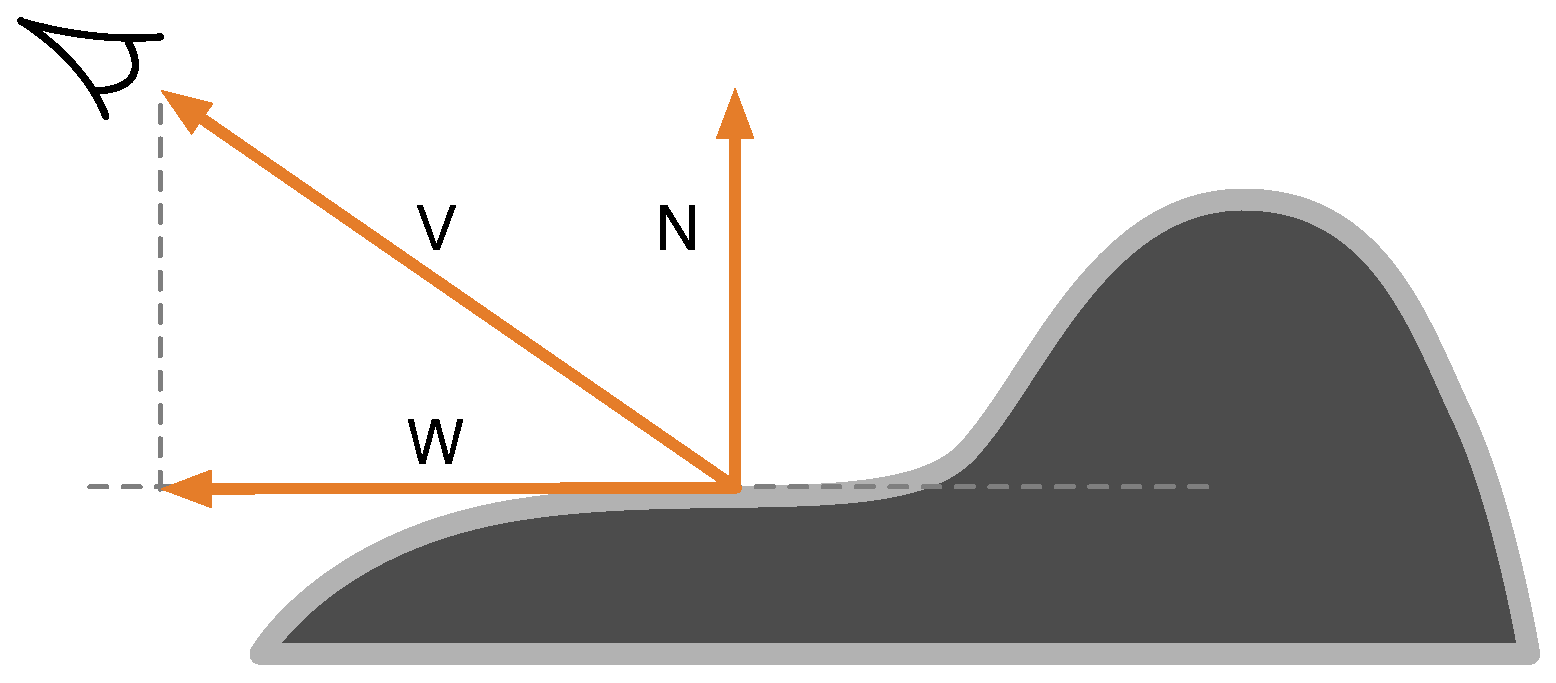
\includegraphics[width=0.9\linewidth]{suggestive_contour_definition}
    \caption[\scon{}的定义]{\label{fig:suggestive_contour_definition}
    \scon{}的定义。其中$N$表示表面法线,$V$表示视线方向,$W$表示$V$在切平面上的投影。}
\end{figure}

其中$\phi$表示绕主方向$D_1$转过的角度。该公式也被称为法线曲率的欧拉公式,它表示了任意方向上的曲率是关于两个主曲率的一个函数。\scon{}的定义和法向曲率直接相关。从比较直观的角度来看,\scon{}表示三维模型表面上$N\cdot{V}$在$W$方向上的局部最小值,其中$W$表示$V$在切平面的投影,\autoref{fig:suggestive_contour_definition}展示了表面上某点属于\scon{}的一个例子。换言之,要找到\scon{},其实就是要找到$N\cdot{V}$的导数的零点,并且保证此处的二阶导数的值为正。而$N\cdot{V}$在$W$方向上的导数等于$W$方向上的法向曲率$\kappa_r$乘以一个常数,推导如下:

\begin{align}
    D_w(N\cdot(V)) &= D_w{N}\cdot{V} + N\cdot{D_w{V}} \\
                   &= D_w{N}\cdot{W} \\
                   &= \rm II(W, W) \\
                   &= (W\cdot{W})\kappa_r
\end{align}
  
在上述推导中,第一行是使用链式法则展开的结果,其中第一个项中的$D_w{N}$表示$N$在$W$上的导数,它的方向必然是在切平面上,所以可以把$D_w{N}\cdot{V}$替换为$D_w{N}\cdot{W}$,而第二项中的$D_w{V}$也必然垂直于$N$,因此直接消去。所以,从公式的角度,\scon{}的定义如下:

\begin{align}
  \kappa_r &= 0\\
  D_w\kappa_r &> 0
\end{align}

其中,$W$方向上的$\kappa_r$也被称为表面上一点的径向曲率(radial curvature)。$D_w\kappa_r$表示$\kappa_r$在方向$W$上的导数,由于需要保证是局部极小值,所以需要保证二阶导数大于零。类似地,$D_w\kappa_r$可以表示为关于$W$的形式:

\begin{equation}
    D_w\kappa_r = C(W, W, W)
\end{equation}

其中$C$是一个对称的三阶张量,可以用4个常数来表示。

\section{相关工作}

\subsection{轮廓线的绘制算法}

在计算机图形学领域,研究者们针对不同的应用提出了多种多样的轮廓线绘制算法。大致地,可以将目前常用的轮廓线绘制算法分为两类,一类是基于图像处理的绘制算法,另一类是轮廓线直接检测的绘制算法。

基于图像处理的轮廓线绘制算法实现起来较为简单直接,其核心思想是利用G缓冲(G-buffer)中存储的信息在图像空间判断是否出现轮廓线。G缓冲是延迟着色\cite{duluk2004deferred}的绘制流程的中间产物。在延迟着色的第一个阶段中,场景会被绘制一次但不进行着色,只是将三维模型的位置、法向等信息存储到一个图像空间的缓冲中,这个缓冲被成为G缓冲。在延迟着色的第二个阶段,再通过一个全屏后处理以G缓冲作为输入完成着色。Decaudin等人拓展了G缓冲的使用方法,在他们的工作\cite{decaudin1996cartoon}中,以G缓冲中的法线和深度信息组成输入,利用索贝尔算子\cite{gao2010improved}等图像滤波的方法进行边缘检测,从而绘制出轮廓线。基于图像处理的方法的好处在于适用性强,只需要一个全屏后处理即可完成,而且可以同时在后处理中完成其他类型的线条的绘制,在效率上有着很大的优势。但是,在绘制质量上,基于图像处理的方法并不占优。该方法的缺陷在于:在深度变化较小或者法线变化较小的区域,例如放在桌子上的纸面的边界,该方法并不能正确地绘制出轮廓线。另外,索贝尔算子等边缘检测方法大多不是良定义的,其最终效果的好坏一定程度上依赖于一些输入参数的人工调节,效果并不稳定。

相比于基于图像处理的轮廓线绘制算法存在上述的各种缺点,而轮廓线的直接检测的绘制算法在绘制质量以及可控性上明显要更好一些。轮廓线的直接检测指的是在世界空间或对象空间直接根据三维模型的几何信息检测出轮廓线,这一类绘制算法能够对线条进行更加精细的操作,方便对线条进行进一步的风格化绘制。轮廓线的直接检测较早的做法\cite{marshall2001cartoon}描述如下:遍历三维模型的三角形网格上的每一条边,判断这些边是否属于轮廓线并保存对应的信息。尽管可以通过排除同一个面的边或者保存每个面的点积等方法来进行优化,但是由于每一帧都要对于新的视点重新遍历三角形网格,这种方法的计算耗时依然很大。Decaudin等人提出了一个更高效的做法\cite{decaudin1996cartoon}。他们的核心想法是,假设帧与帧之间视点和物体之间发生的移动较少,可以认为上一帧检测的轮廓线在这一帧依然会是轮廓线。他们通过计算上述的移动距离从而避免每一帧的重新遍历所需的计算量,相较于前者的方法在效率上获得来很大的提升。由于检测过程中可以精确地获取轮廓线的信息,轮廓线的直接检测对进一步的风格化处理非常有利,但是相较于基于图像处理的方法而言,实现上较为复杂。不过,随着现代GPU绘制流水线的发展,可编程着色器越来越灵活,轮廓线的直接检测方法也可以实现地非常简单而又高效。目前比较高效的实现方法是使用可编程着色器中的几何着色器(geometry shader)来完成轮廓线的直接检测,这样可以充分利用GPU的并行计算的高性能,并摆脱传统方法中CPU与GPU的交互,直接在绘制流水线中完成轮廓线的绘制,使得绘制效率大大提升。本文正是通过编写几何着色器来高效地实现\con{}以及\scon{}的绘制算法,在下文的第二章中会进行相关的具体说明。

\begin{figure}[tbh]
    \centering
    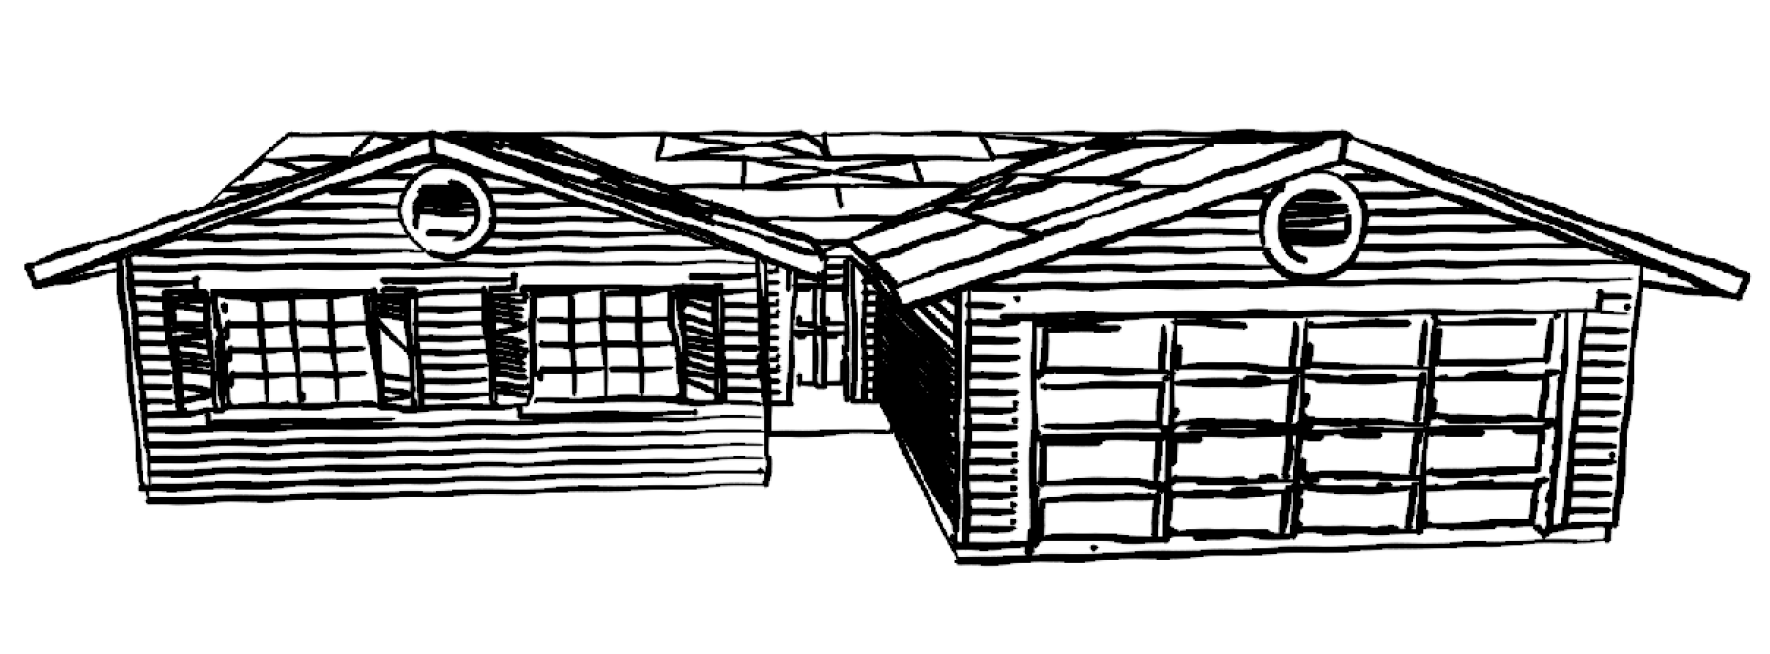
\includegraphics[width=\linewidth]{stylized_house}
    \caption[使用风格化线条绘制的建筑物]{\label{fig:stylized_house}
    使用风格化线条绘制的建筑物\cite{northrup2000artistic}}
\end{figure}

需要特别指出的是,虽然线绘制本身属于非真实感绘制或者风格化绘制的其中一种技术,但是关于线条的进一步风格化也是一项独立的研究课题:风格化线条(stylized line)。一般的线绘制只是涉及如何利用绘制流水线构建给定定义的线条并进行快速的绘制,而风格化线条指的是在此基础上对线条的外形、着色进行艺术风格的表达,例如使线条呈现出毛笔、笔刷等绘画工具的质感。\autoref{fig:stylized_house}展示了风格化线条的一个例子。Northrup等人在\cite{northrup2000artistic}中提出了对轮廓线进行进一步风格化的方法。在他们的方法中,先按照已有的方法找到所有轮廓线的线段,然后处理这些线段之间的重叠并将在图像空间线段连接成连续的长线。接着,再以这些长线为对象进行绘制,在绘制的过程中将线条沿着法线方向展开为四边形,使得最后在着色阶段可以贴上纹理进行绘制,进而表现出特定的笔刷效果。Isenberg等人在\cite{isenberg2002stylizing}中提出了改进的方法。在前人的方法中,线段之间是通过在图像空间搜索相邻的端点来建立连接的,而Isenberg等人的方法将这一步骤改进为利用三维模型本身的三角形的邻接关系来寻找相邻的端点,使得绘制速度获得了很大的提升。

\subsection{\stc{}\npr{}}

线绘制属于\npr{}技术中的一种。一般而言,\npr{}的相关研究只关注如何解决单目绘制下的问题。不过,近年来\npr{}和双目绘制的结合越来越受到关注,出现了不少关于\npr{}在双目绘制下的问题的研究。为了避免双目绘制下基于笔画的图像风格化算法\cite{hertzmann1998painterly}带来的问题,Northam等人\cite{northam2012consistent,northam2013stereoscopic}提出了将左眼和右眼的画面分离成离散的差异层的方法。在得到左眼和右眼对应的差异层后,他们提出的方法将对应的层组合起来再作进一步的基于笔画的风格化,从而得到\stc{}的图像。\autoref{fig:disparity}展示了用他们提出的方法得到的一个结果。

\begin{figure}[tbh]
    \centering
    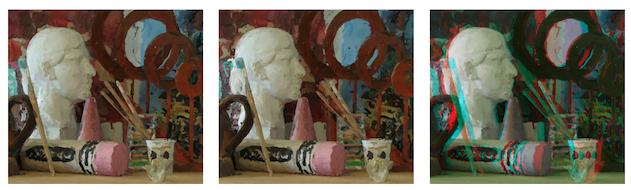
\includegraphics[width=\linewidth]{disparity}
    \caption[\stc{}基于笔画的图像风格化]{\label{fig:disparity}
    \stc{}基于笔画的图像风格化\cite{northam2012consistent}}
\end{figure}

除了基于图像的风格化算法,基于三维模型的线绘制在双目绘制下的问题也有一定的研究。Kim等人在他们的工作中具体定义了关于轮廓线的\stc{}概念,并提出了在多个视点上检查\ec{}上的对应轮廓点的的方法来保证轮廓线的\stcy{},该方法对于\scon{}也同样适用。此外,Bukenberger等人在近年提出了一个新的方法\cite{bukenberger2018stereo}来解决\stc{}\con{}绘制这个问题。与前者在图像空间中处理的方法相比,他们的方法着力于利用物体空间的信息来解决这个问题。他们的方法首先绘制出不同给定视点下的\con{}的结果并以物体空间的形式存储下来,接着利用这些信息通过插值得出新视点下\stc{}\con{}的图像。

在\stc{}\con{}绘制的基础上,如何做进一步的风格化的问题也得到了关注\cite{northrup2000artistic,kalnins2003coherent} 。Kim等人和Bukenberger等人都在他们各自的工作中提出了对\stc{}的\con{}进行风格化的方法。在获得不同视点下轮廓点的对应关系的基础上,Kim等人在不同视点之间传递风格化参数的方法,从而保证进一步的风格化处理依然保持最后结果是\stc{}。在Bukenberger等人的工作中,进一步的风格化参数由物体的三维表面的一些特征决定,以此来保证结果的时序一致性(temporal coherency)。同样,本文将先就如何实现\stc{}\con{}和\scon{}来进行阐述,然后再描述进一步风格化的解决方法。

\subsection{\ppll{}}

\begin{figure}[tbh]
    \centering
    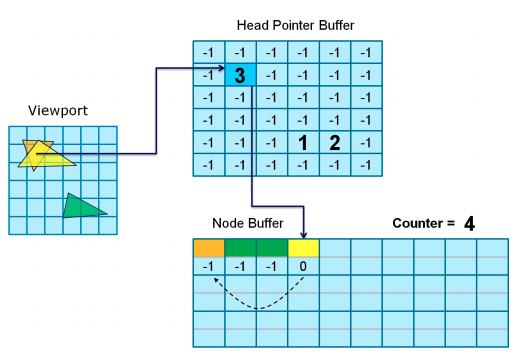
\includegraphics[width=\linewidth]{ppll}
    \caption[\ppll{}所使用的数据结构]{\label{fig:ppll}
    \ppll{}所使用的数据结构\cite{yang2010real}}
\end{figure}

链表是计算机领域中常用的一种数据结构。链表往往用于存储不定长度的数据集合,在各式各样的CPU上的算法上很常见也易于实现,但是在GPU上没有简单直接的实现方法。Yang等人提出了一个高效的方法\cite{yang2010real}来在GPU上构建链表。他们的方法使用一个缓冲来存储所有的链表节点,并使用另一个图像空间的缓冲区来存储逐个像素上的链表头部节点,这些头部节点指向上述第一个缓冲中的用于存储实际信息的节点,\autoref{fig:ppll}展示了他们设计的数据结构。\ppll{}是用来处理逐个像素上的多个片段(fragment)的最具有普适性的工具,一个典型的用例是进行排序无关的透明绘制(order independent transparency)。在一般的绘制流程中,由于深度测试(depth test)的存在以及透明物体做透明度混合(alpha blending)的需要,往往需要在CPU端先对各个三维模型从远到近进行排序,然后按顺序进行绘制,否则会导致远处的透明物体被近处的透明物体所遮挡的错误结果。在Barta等人的工作中\cite{barta2011order},他们提出了用\ppll{}来进行排序无关的透明绘制的方法。在他们的方法中,不需要在CPU端对三维模型进行排序,而是先将三维模型绘制到\ppll{}上,其中每个像素存储了多个来自于不同的三维模型的片段颜色以及对应的距离,然后通过另外一个全屏后处理对\ppll{}上每个像素的多个片段按照距离进行排序并计算出透明度混合的结果。由于只需要在片段着色器阶段对多个片段进行排序,整个过程可以完全在GPU中实现,所以相比一般在CPU端进行排序的方法效率更高,而且更加灵活。

为了避免轮廓点的重叠带来的问题,本文设计的方法使用\ppll{}来访问位于同一个像素点上的多个不同轮廓点的数据。由于本文设计的方法只需要对轮廓点建立链表,而这些轮廓点只占整体画面的一小部分,所以\ppll{}的内存占用量并不大。